\section{Introducción}
El Modelo OSI es una referencia mediante la cual se estandariza la forma en como debe llevarse a cabo la comunicación. Aborda todos los procesos necesarios para una comunicación efectiva y divide estos procesos en grupos lógicos llamados capas. 
Este modelo se basa en una propuesta desarrollada por la Organización Internacional de Normalización (ISO) como un primer paso hacia la estandarización internacional de los protocolos utilizados en las diversas capas.
\\${ }$\\
El modelo se denomina Modelo de referencia OSI (Open Systems Interconnection) porque trata de conectar sistemas abiertos, es decir, sistemas que están abiertos para la comunicación con otro sistema. 
\\ ${ }$\\
De manera concreta podríamos representarlo con el siguiente diagrama:
\begin{figure}[!ht]
\centering
\begin{tikzpicture}
 
   \draw [decorate,decoration={brace,amplitude=10pt},xshift=-5pt,yshift=0pt]
(0.5,0) -- (0.5,2.25) node [black,midway,xshift=-0.8cm] 
{\footnotesize Media };

   \draw [decorate,decoration={brace,amplitude=10pt},xshift=-5pt,yshift=0pt]
(0.5,2.5) -- (0.5,5.75) node [black,midway,xshift=-0.8cm] 
{\footnotesize Host \hspace{0.5cm}};

  \node at (2.5,5.5) (c1)  [wide]   []  {Application};
  \node (c2)  [wide]   [below = 0.1cm of c1]  {Presentation};
  \node (c3)  [wide]   [below = 0.1cm of c2]  {Session};
  \node (c4)  [wide0]   [below = 0.1cm of c3]  {Transport};
  \node (c5)  [wide2]   [below = 0.1cm of c4]  {Network};
  \node (c6)  [wide3]   [below = 0.1cm of c5]  {Data Link};
  \node (c7)  [wide4]   [below = 0.1cm of c6]  {Physical};
  
  \begin{pgfonlayer}{background}
   
  \end{pgfonlayer}
  

\end{tikzpicture}
\caption{Diagrama que representa el Modelo OSI}
\end{figure}
\\
Donde las capas que pertenecen al \textbf{Medio} son responsables de ver que la información llegue al destino para el que fue destinada y las capas que pertenecen al \textbf{Host} son responsables por la entrega de datos entre computadoras.
\\$ { }$\\
Los principios que se aplicaron para llegar a las siete capas se pueden resumir brevemente de la siguiente manera:
\begin{itemize}
\item Se debe crear una capa donde se necesita una abstracción diferente.
\item Cada capa debe tener una función bien definida.
\item La función de cada capa debe elegirse teniendo en cuenta la definición de protocolos estandarizados internacionalmente.
\end{itemize}
\subsection{Capas del Modelo OSI}



\subsubsection{Aplicación (Application)}
Este es el nivel con el que el usuario a menudo interactúa. Aquí es donde los datos se convierten en sitios web, programas de chat, etc.

\subsubsection{Presentación (Presentation)}
Aquí es donde los datos de la aplicación se empaquetan o desempaquetan, listos para su uso por la aplicación en ejecución. La conversión de protocolos, el cifrado / descifrado y la expansión de gráficos tienen lugar aquí.
\subsubsection{Sesión (Session)}
Esta es la capa responsable de abrir y cerrar la comunicación entre los dos dispositivos. El tiempo entre el momento en que la comunicación se abre y se cierra se conoce como sesión.
\subsubsection{Transporte (Transport)}
Esta capa se ocupa principalmente de la confiabilidad (seguridad como cifrado / descifrado, firewall, etc.), el mantenimiento del flujo de paquetes al reducir la congestión y realiza una verificación de errores que garantiza que los datos transmitidos estén completos.
\subsubsection{Red (Network)}
La capa de red divide los segmentos de la capa de transporte en unidades más pequeñas, llamadas paquetes, en el dispositivo del remitente, y vuelve a ensamblar estos paquetes en el dispositivo receptor. La capa de red también encuentra la mejor ruta física para que los datos lleguen a su destino; Esto se conoce como enrutamiento.
\subsubsection{Enlace (Data Link)}
Esta capa muy similar a la capa de red, excepto que la capa de enlace de datos facilita la transferencia de datos entre dos dispositivos en la misma red. Su función principal de esta capa es proporcionar un método mediante el cual la información de la red se descompone en tramas y se transmite a través de la capa física. Esta capa también es responsable de la detección y corrección de algunos errores.

\subsubsection{Física (Physical)}
Esta capa incluye el equipo físico involucrado en la transferencia de datos, como los cables y conmutadores.
Sus funciones son convertir señales en bits, que pueden ser utilizados por otra capa y ajustar la señal para permitir que varios usuarios usen la misma conexión. También especifica cómo un dispositivo envía y recibe información.
\subsection{Funcionamiento de las 7 Capas}
Para explicar como funciona este modelo necesitamos partir desde el momento que se interactúa con algun programa o sitio, digamos que queremos enviar un correo con mensaje y unos archivos, a esto se le conoce como la capa de Aplicación, al hacer click en enviar esta información se empaqueta, y se encripta esta sería la capa de Presentación; una vez empaquetado los datos, se ''abre'' una sesión, es decir, se establece un enlace entre dos computadoras, esta es la capa de Sesion, una vez establecidad la sesion, la capa de transporte verifica que hasta esta etapa no haya errores o que los datos no sean corruptos, y en caso de serlos puede eliminarlos o devolverlos de donde vienen. Una vez atravesada la capa de transporte viene la capa de Red, aqui la información se divide en partes mas pequeñas y se les coloca la fuente de los datos y el destino de estos (dirección IP), acto seguido viene la capa de enlace, esta capa finalmente es la que despacha los datos libres de errores tranformándolos en tramas, y estas van a la capa Física para convetirse en señales que viajan a travez de los cables hasta el destino, en el destino este procedimiento es ejecutado de manera inversa, convirtiendo las señales en tramas, reconstruyendo estas para formar lo paquetes, revisando que los paquetes no esten corruptos y sean seguros, estableciendo una sesión, desempaquetando lo datos, desencriptandolos para finalmente entregarlos a la aplicación del otro lado.

\begin{figure}[!ht]
\centering
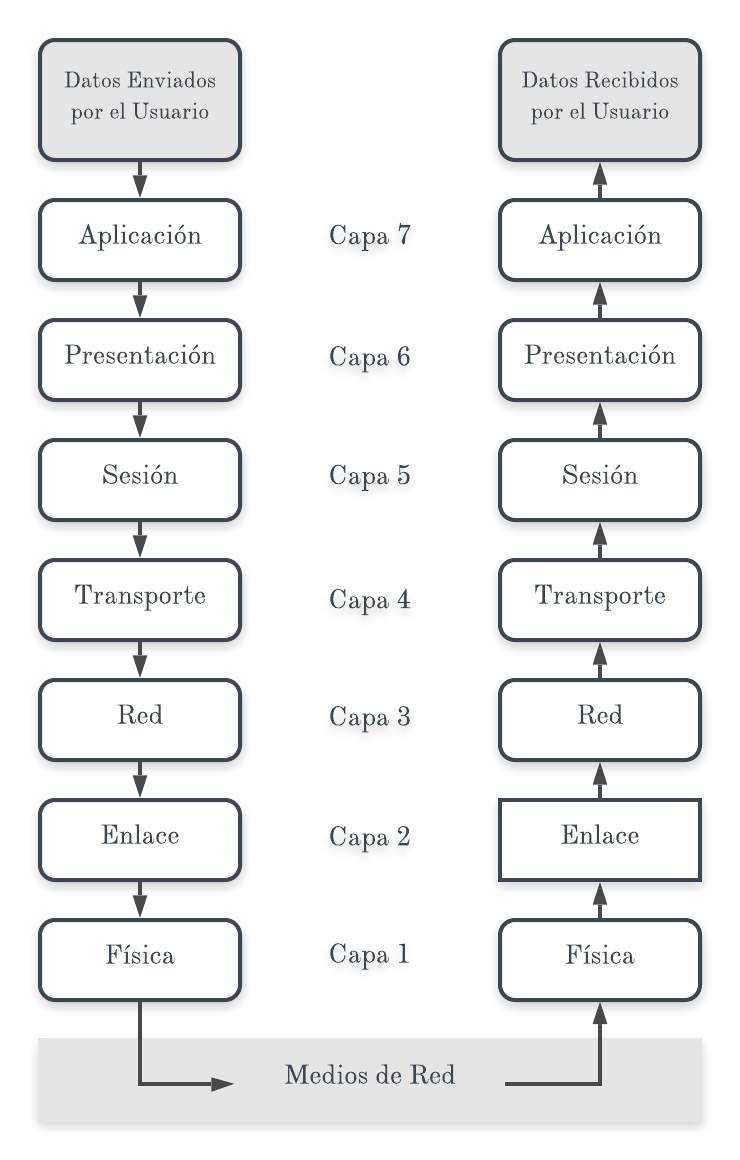
\includegraphics[scale=0.25]{OSI}
\caption{Diagrama que muestra como es que se transmiten los datos}
\end{figure}
\pagebreak


\begin{thebibliography}{9}
\bibitem{Tanen} 
Tanenbaum, Andrew S., and D Wetherall. Computer networks. Boston: Pearson Prentice Hall, 2011. Print.
\bibitem{Neil} 
Briscoe, Neil. Understanding The OSI 7-Layer Model. 2002.
\bibitem{OJCTT} 
Gaurav Bora, Saurabh Bora, Shivendra Singh, Sheikh Mohamad Arsalan. OSI Reference Model: An Overview. International Journal of Computer Trends and Technology, Volume 7 Number 4. 2014.


\end{thebibliography}

